\chapter{Stato dell'arte}
\label{StatoArte}
\thispagestyle{empty}

%\begin{quotation}
%{\footnotesize
%\noindent{\emph{``Terence: Rotta a nord con circospezione \\
%Bud: Ehi, gli ordini li do io qui!\\
%Terence: Ok, comante\\
%Bud: Rotta a nord\\
%Terence: Soltanto?\\
%Bud: Con circospezione!''}
%}
%\begin{flushright}
%Chi Trova un Amico Trova un Tesoro
%\end{flushright}
%}
%\end{quotation}
\vspace{0.5cm}

\noindent In questo capitolo elenchiamo quelle che sono le principali tecniche, presenti nella letteratura scientifica, utilizzate per identificare tentativi di manomissione su camere di videosorveglianza. 
\section{Modello della camera}

\section{Monitoraggio video: concetti e terminologia}
Prima di concentrarci sul problema del tampering detection, definiamo, i concetti e i termini che verranno utilizzati nel seguito della trattazione.\\
Lo scenario che consideriamo \`e quello di una camera che deve riprendere una particolare \textit{\gls{scena}}.
\begin{figure}
	\centering
	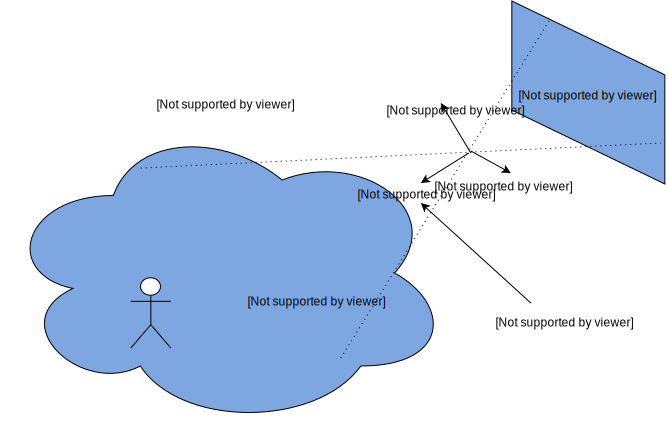
\includegraphics[width=12cm]{./pictures/videoMonitoring}
	\caption{Sistema di monitoraggio video}
	\label{fig:videoMonitoring}
\end{figure}
\noindent 
La posizione e l'orientamento della camera determinano l'\textit{\gls{inquadratura}} della scena.
L'acquisizione, da parte della camera, della scena nell'istante di tempo $i$ viene definita \textit{immagine} o \textit{frame} i-esimo.
La figura \ref{fig:videoMonitoring} illustra questi concetti.\\
Nel seguito della trattazione useremo una specifica terminologia.
Indicheremo con $\mathcal{X}$ l'insieme dei \textit{pixel} costituenti l'immagine acquisita dalla camera,
\[ \mathcal{X} \subset \mathbb{N}^2, \]
e con $x \in \mathcal{X}$ il singolo pixel.
Quando vorremo considerare il frame acquisito all'istante di tempo $i$, useremo $z_i$, con $i=1,\dots , \infty$. 
In particolare, per indicare il valore della \textit{luminosit\`a} del pixel $x$ per il frame $i$-esimo, useremo il termine $z_i(x)$, con 
\[ z_i(x) \in [0, 255]. \]
\section{Tampering Detection}
In un'applicazione di monitoraggio video consideriamo che la camera, in condizioni di funzionamento ottimale, mantenga la stessa inquadratura nel tempo e che sia in grado di acquisire, in maniera nitida, tutti gli elementi di interesse presenti nella scena.
Definiamo \gls{tampering} un qualsiasi evento che determina un cambio di inquadratura o che non permette la corretta acquisizione di parte o totalit\`a della scena.
Possiamo classificare gli eventi di tampering in quattro categorie:
\begin{itemize}
	\item sfocature,
	\item spostamenti della camera,
	\item occlusioni dell'obiettivo,
	\item guasti della camera.
\end{itemize}
Nei moderni sistemi di videosorveglianza troviamo spesso algoritmi utilizzati per identificare particolari eventi all'interno della scena ripresa dalla camera. 
Ad esempio \`e possibile avere un software in grado di identificare le targhe delle automobili che superano il limite di velocit\`a, oppure la presenza di oggetti incustoditi in una stazione \cite{Targhe}.
Affinch\'e questi algoritmi funzionino correttamente, \`e importante che l'\textit{affidabilit\`a} del sistema di acquisizione sia preservata.
Per fare questo la letteratura scientifica offre molte tecniche che permettano l'identificazione automatica di eventi in grado di compromettere la corretta ripresa della scena da parte della videocamera.
Possiamo dividere le principali tecniche di tampering detection in due categorie: 
\begin{itemize}
	\item tecniche basate su confronto di background,
	\item tecniche basate su monitoraggio sequenziale.
\end{itemize}
\subsection{Tecniche basate su confronto di background}
Nella maggior parte dei lavori dedicati a questo problema, il concetto principale consiste nel confrontare ciascun frame con un modello che viene calcolato utilizzando i frame precedenti.
Tale modello \`e ampiamente utilizzato in vari ambiti di visione artificiale e prende il nome di \textit{modello di background}.
Un metodo generale di calcolo del background \`e presentato in \cite{aksay2007camera}.
Indichiamo con $z_i(x)$ il valore, nel pixel $x$, della luminosit\`a nell'$i$-esimo frame.
Il valore del modello di background \`e calcolato in maniera ricorsiva secondo la seguente formula:

\[
\label{eq:background}
B_{i + 1}(x)=\left\{ \begin{array} {lcl}
aB_i(x)+ (1-a)z_i(x) & \mbox{, se} & |z_i(x) - z_{i-1}(x)|\leq T_i(x) \\
B_i(x) & \mbox{, se} & |z_i(x) - z_{i-1}(x)|>T_i(x)\end{array} \right. ,
\]

dove $0 < a < 1$ \`e chiamato \textit{parametro di aggiornamento} (\textit{update parameter}) e $T_i(x)$ \`e una soglia che permette di identificare un cambiamento sostanziale di luminosit\`a nel pixel $(x)$. 
 Questa soglia viene aggiornata in maniera ricorsiva secondo la seguente formula:
  \[
  \label{eq:backgroundThreshUpd}
  T_{i + 1}(x)=\left\{ \begin{array} {lcl}
  aT_i(x)+ (1-a)(c |z_i(x) - B_i(x)|) & \mbox{, se} & |z_i(x) - z_{i-1}(x)|\leq T_i(x) \\
  T_i(x) & \mbox{, se} & |z_i(x) - z_{i-1}(x)|>T_i(x) \end{array} \right. ,
  \]
  dove $c > 1$ e $0<a<1$.
  Lo stesso modello viene applicato in altri lavori (\cite{saglam2009real}, \cite{tsesmelis2013tamper}), mentre una variante molto usata consiste nell'estrarre il modello di background a partire dall'\textit{estrazione dei contorni} da ciascun frame (\cite{harasse2004automated}, \cite{gil2007automatic}).
  Un approccio diverso, ma comunque riconducibile allo stesso filone, lo troviamo in \cite{ribnick2006real}, dove il background \`e sostituito da un \textit{buffer} contenente gli ultimi $n$ frame acquisiti dalla camera, che vengono confrontati con l'ultima osservazione per identificare eventi di tamepering.
\subsubsection{Identificazione di occlusioni}
L'evento di occlusione avviene quando un oggetto opaco viene posto vicino alla camera, in modo da coprire la scena ripresa.
In \cite{aksay2007camera} e \cite{saglam2009real} questo evento \`e associato a un cambiamento nella struttura dell'\textit{istogramma} del frame occluso rispetto a quello del background.
Infatti, nel caso di occlusioni, i valori dell'istogramma tendono a concentrarsi in un intervallo molto ristretto, verso i livelli pi\`u bassi della scala di grigi.\\
Un approccio simile \`e presente in \cite{harasse2004automated}, \cite{gil2007automatic} e \cite{ellwart2012camera}, in cui l'evento di occlusione \`e associato a un abbassamento dell'\textit{entropia}:
 \[
 \label{eq:entropy}
 E=-\sum_{k}p_k\ln(p_k) ,
 \]
 dove $p_k$ rappresenta la probabilit\`a che il livello di grigio $k$ sia presente all'interno dell'immagine. 
\subsubsection{Identificazione di spostamenti della camera}
Quando viene spostata la camera, in modo cambi l'inquadratura della scena, l'immagine di background $B_i$ viene lentamente aggiornato in modo da riflettere i cambiamenti avvenuti nei frame. 
In \cite{saglam2009real} il metodo proposto per identificare uno spostamento della camera consiste nel confrontare l'immagine di background $B_i$ con $B_{i-k}$, ovvero con un secondo modello \textit{ritardato} di $k$ frame, dove $k \in \mathbb{Z}^+$.
L'approccio consiste nel calcolare un \textit{valore di proporzione} $P$, ottenuto dal confronto tra i due modelli:
\[
\label{eq:displEqSaglam}
P=\left\{ \begin{array} {lcl}
P+1 & \mbox{, se} & B_i(x) \neq B_{n-k}(x) \\
P & \mbox{, se} & B_i(x) = B_{n-k}(x) \end{array} \right. .
\]
Lo spostamento della camera viene identificato quando $P > Th K$, dove $0<Th<1$ \`e un valore di soglia scelto in base alla sensibilit\`a che si vuole dare all'algoritmo e $K$ \`e il numero totale di pixel dell'immagine.\\
Un altro approccio \`e quello di utilizzare tecniche di \textit{block matching}.
In \cite{gil2007automatic} e \cite{harasse2004automated} il confronto viene fatto utilizzando la formula \textit{zero-mean normalized cross correlation} (ZNCC) \cite{roma2002comparative}:
\[
ZNCC_i(m) = \frac{\sum_{x \in \mathcal{X}}(B_{i-1}(x)- \mu_{B_{i-1}})(z_i(x+m)-\mu_{z_i})}{\sigma_{B_{i-1}} \sigma_{z_i}},
\]
dove $\mu_{z_i}$ e $\sigma_{z_i}$ rappresentano la media e la deviazione standard della luminosit\`a nell'immagine $z_i$.
Un'altra cifra di merito, utilizzata in \cite{ellwart2012camera}, \`e la \textit{minimum squared difference} (MSD):
\[
MSD = \frac{1}{K}\sum_{x \in \mathcal{X}}(z_i - B_i)^2
\]
L'algoritmo di block matching fornisce due parametri:
il primo parametro, $m$, indica il \textit{vettore della traslazione} tra il background e il frame corrente, mentre il secondo parametro \`e lo ZNCC relativo a quel vettore.
Lo spostamento viene individuato quando il vettore $m$ ha una lunghezza minima e lo ZNCC corrispondente supera una certa soglia.
Un metodo simile viene utilizzato anche in \cite{kryjak2012fpga}, con la differenza che, invece di analizzare la correlazione dei pixel, viene analizzata quella degli istogrammi. 
\subsubsection{Identificazione di sfocature} 
La conseguenza di un evento di sfocatura \`e la perdita di dettagli nell'immagine.
In \cite{aksay2007camera} e \cite{saglam2009real} questo fenomeno \`e associato a una diminuzione dell'energia ad alta frequenza. 
Per analizzare questo cambiamento, \cite{aksay2007camera} confronta ciascun frame con il background nel dominio delle \textit{wavelet} \cite{mallat1989theory}, mentre \cite{saglam2009real} utilizza il dominio della \textit{trasformata di Fourier} \cite{bracewell1978fourier}.
\begin{figure}
	\centering
	\begin{subfigure}[]
		{\label{fig:defocusNormale} 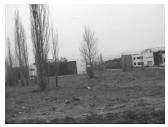
\includegraphics[width = 5cm]{./pictures/normale}}
	\end{subfigure}
	\begin{subfigure}[]
		{\label{fig:defocusNormaleFourier} 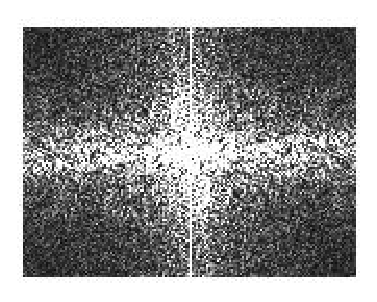
\includegraphics[width = 5cm]{./pictures/normale-fourier}}
	\end{subfigure}
	\begin{subfigure}[]
		{\label{fig:defocusSfocato} 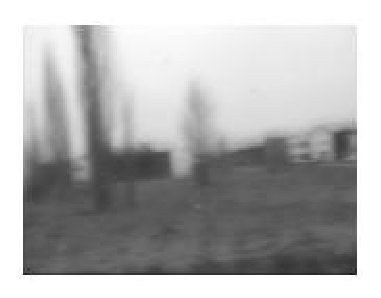
\includegraphics[width = 5cm]{./pictures/sfocato}}
	\end{subfigure}
	\begin{subfigure}[]
		{\label{fig:defocusSfocatoFourier} 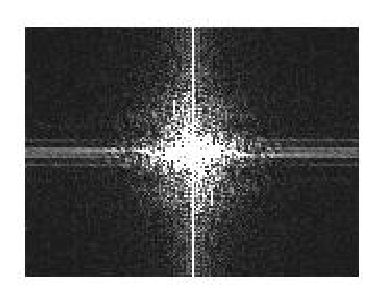
\includegraphics[width = 5cm]{./pictures/sfocato-fourier}}
	\end{subfigure}
	\caption{Comportamento della trasformata di Fourier nel caso di sfocatura}
	\label{fig:fourier}
\end{figure}
Nella figura \ref{fig:fourier} vediamo un esempio di come si comporta la trasformata di Fourier nel caso di sfocature: 
nel passaggio da un frame nitido (Fig. \ref{fig:defocusNormale}) a uno sfocato (Fig. \ref{fig:defocusSfocato}) abbiamo un crollo delle componenti ad alta frequenza nelle trasformate di Fourier (rispettivamente Fig. \ref{fig:defocusNormaleFourier} e Fig. \ref{fig:defocusSfocatoFourier}).
L'evento di tampering viene individuato quando l'\textit{energia media} della trasformata di Fourier (o di quella wavelet) del frame corrente $E_{HF}(z_i)$ \`e $Th$ volte minore di quella del background $E_{HF}(B_i)$:
\[E_{HF}(z_i)\leq Th E_{HF}(B_i),\]
dove $0<Th<1$ \`e  un valore di soglia scelto in base alla sensibilit\`a che si vuole dare all'algoritmo.\\
Un altro approccio consiste nell'analizzare la perdita di dettagli confrontando i contorni (\textit{edges}) del frame corrente con quelli del background.
Questo metodo, utilizzato in \cite{ellwart2012camera}, \cite{gil2007automatic}, \cite{harasse2004automated} e \cite{kryjak2012fpga}, consiste nell'estrarre i contorni dalle immagini secondo il metodo di Sobel \cite{sobel19683x3} o di Canny \cite{canny1986computational}, e confrontare il numero di pixel dei contorni con quelli del background. 
Quando il numero di pixel dei contorni del frame corrente $\sum edges(z_i)$ \`e $Th$ volte pi\`u piccolo di quello del background $\sum edges(B_i)$:
\[ \sum edges(z_i) \leq Th \sum edges(B_i), \]
dove $0<Th<1$ \`e  un valore di soglia scelto in base alla sensibilit\`a che si vuole dare all'algoritmo.
\subsection{Tecniche basate su monitoraggio sequenziale}
Le tecniche viste finora, come \`e stato detto nel paragrafo precedente, permettono di aggiornare ciascun frame con un modello della scena che viene calcolato in base alle osservazioni precedenti.
Questo approccio risulta fattibile nel caso in cui la camera operi con un framerate \textit{continuo}, solitamente tra i 30 frame per secondo (\textit{fps}) e i 2 fps. 
In questi casi, infatti, possiamo considerare che, tra un frame e il successivo, non avvengano grandi cambiamenti all'interno della scena e non cambi eccessivamente la luminosit\`a media.
\begin{figure}
	\centering
	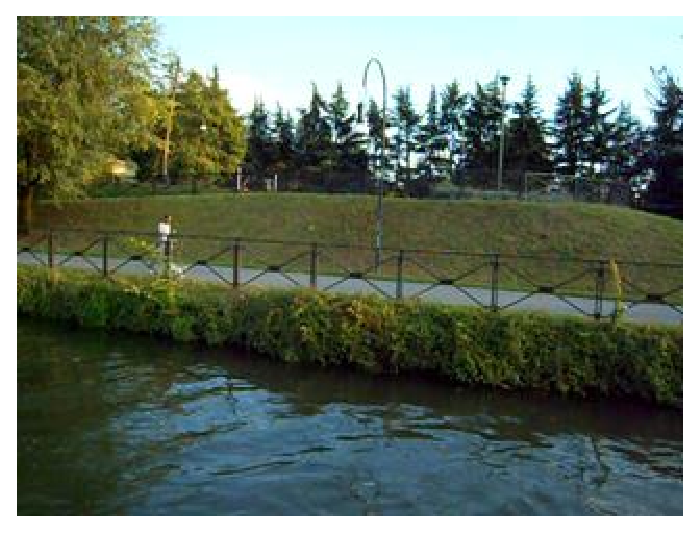
\includegraphics[width = 3cm]{./pictures/FPSalto/img0001}
	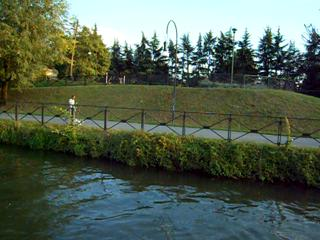
\includegraphics[width = 3cm]{./pictures/FPSalto/img0002}
	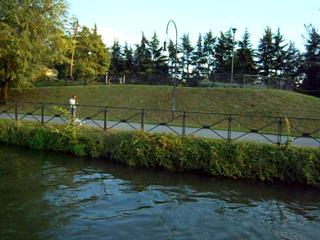
\includegraphics[width = 3cm]{./pictures/FPSalto/img0003}
	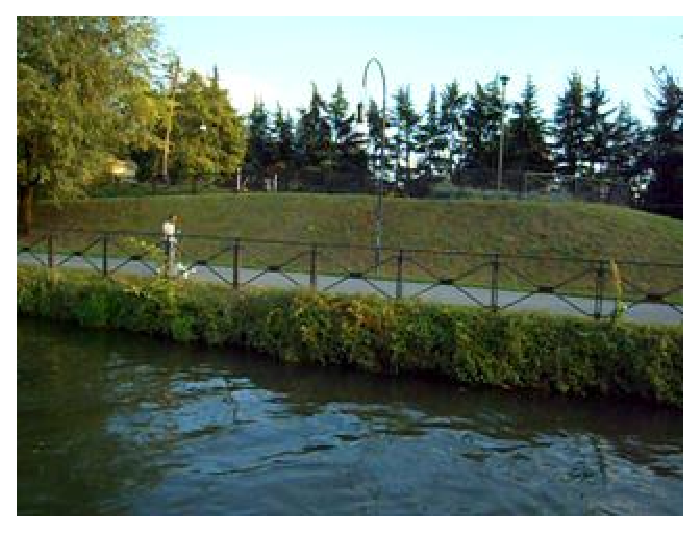
\includegraphics[width = 3cm]{./pictures/FPSalto/img0004}
	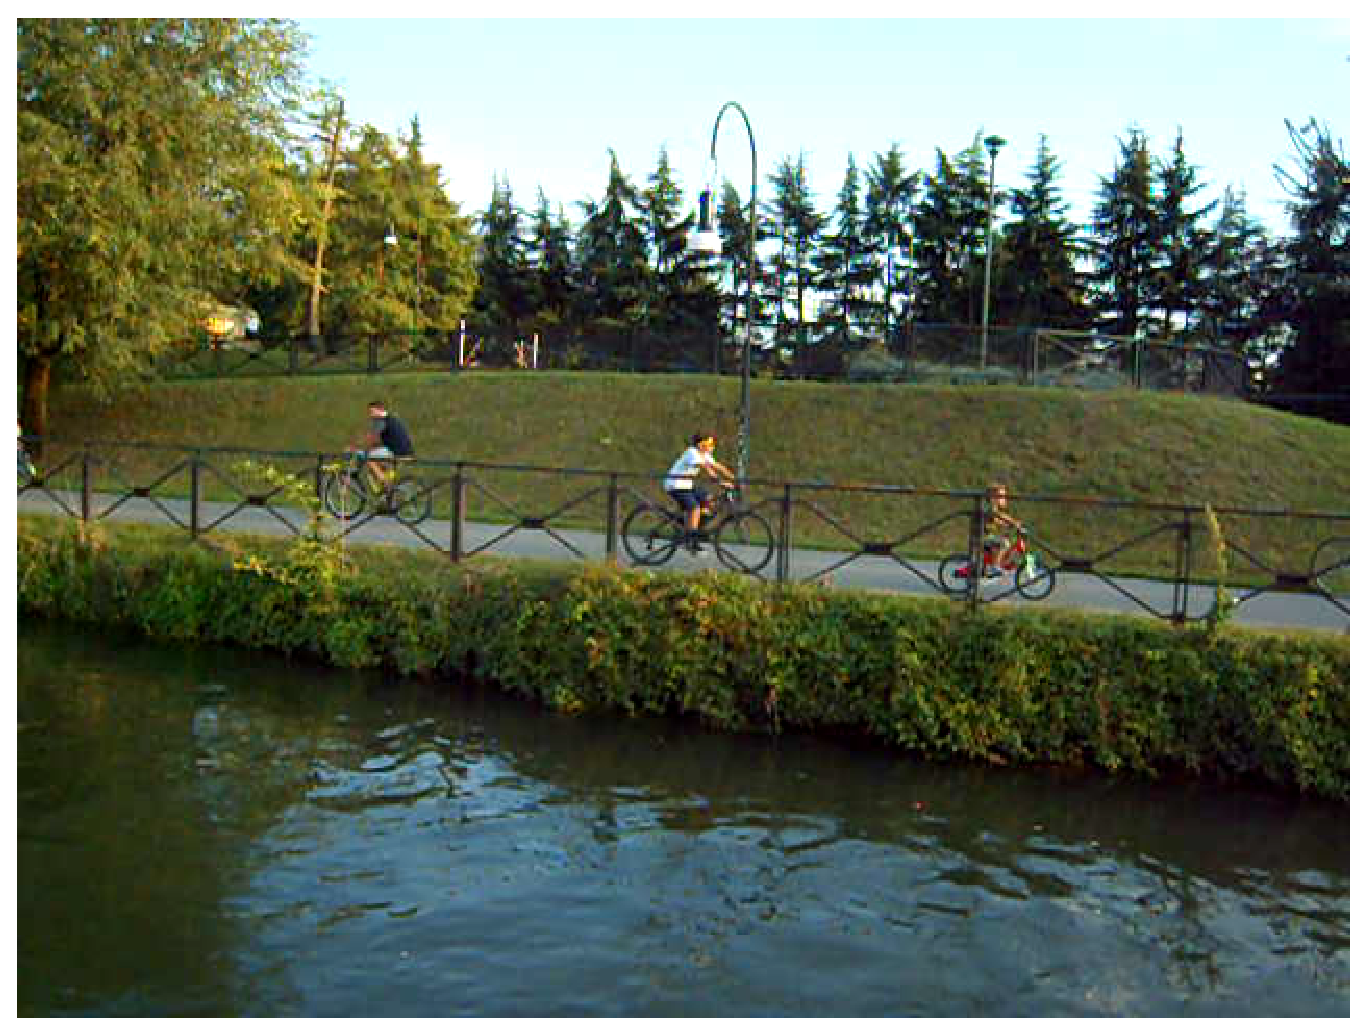
\includegraphics[width = 3cm]{./pictures/FPSalto/img0005}
	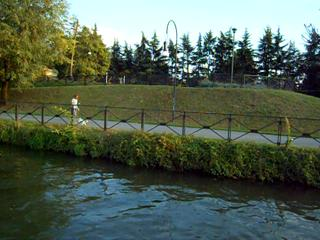
\includegraphics[width = 3cm]{./pictures/FPSalto/img0006}
	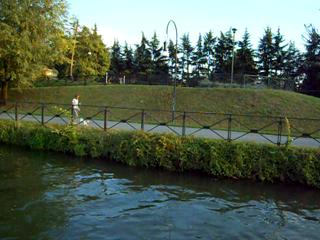
\includegraphics[width = 3cm]{./pictures/FPSalto/img0007}
	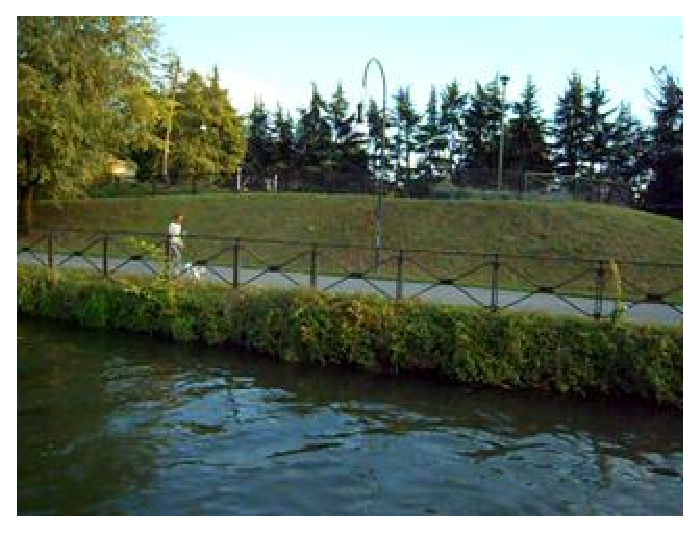
\includegraphics[width = 3cm]{./pictures/FPSalto/img0008}
	\caption{Sequenza di frame acquisiti a 30 fps}
	\label{fig:acquisizioneContinua}
\end{figure}
\begin{figure}
	\centering
	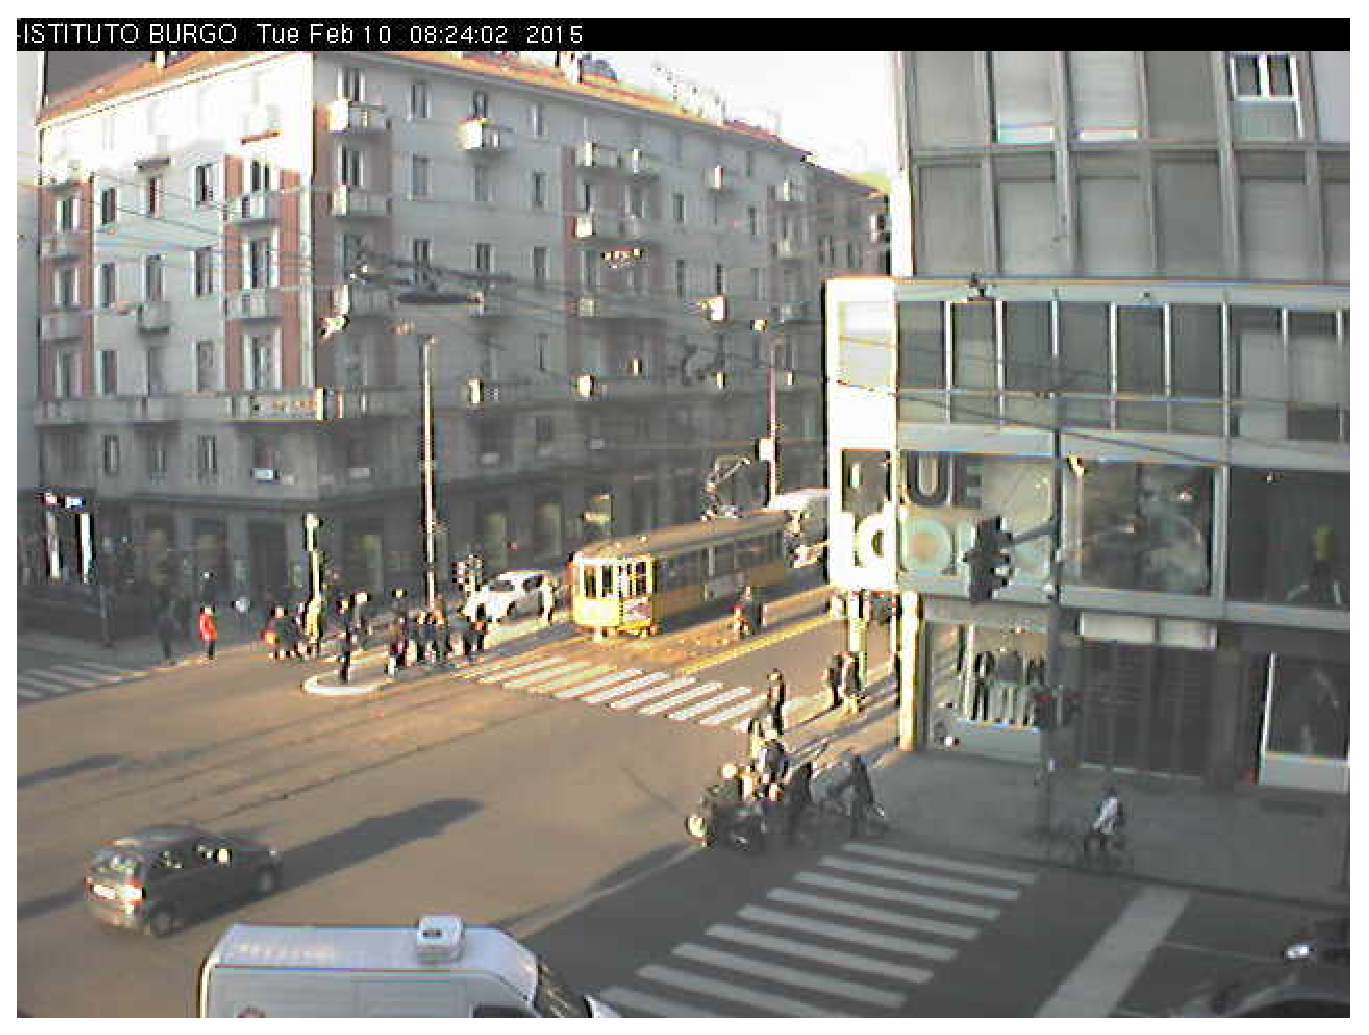
\includegraphics[width = 3cm]{./pictures/FPSbasso/image2691}
	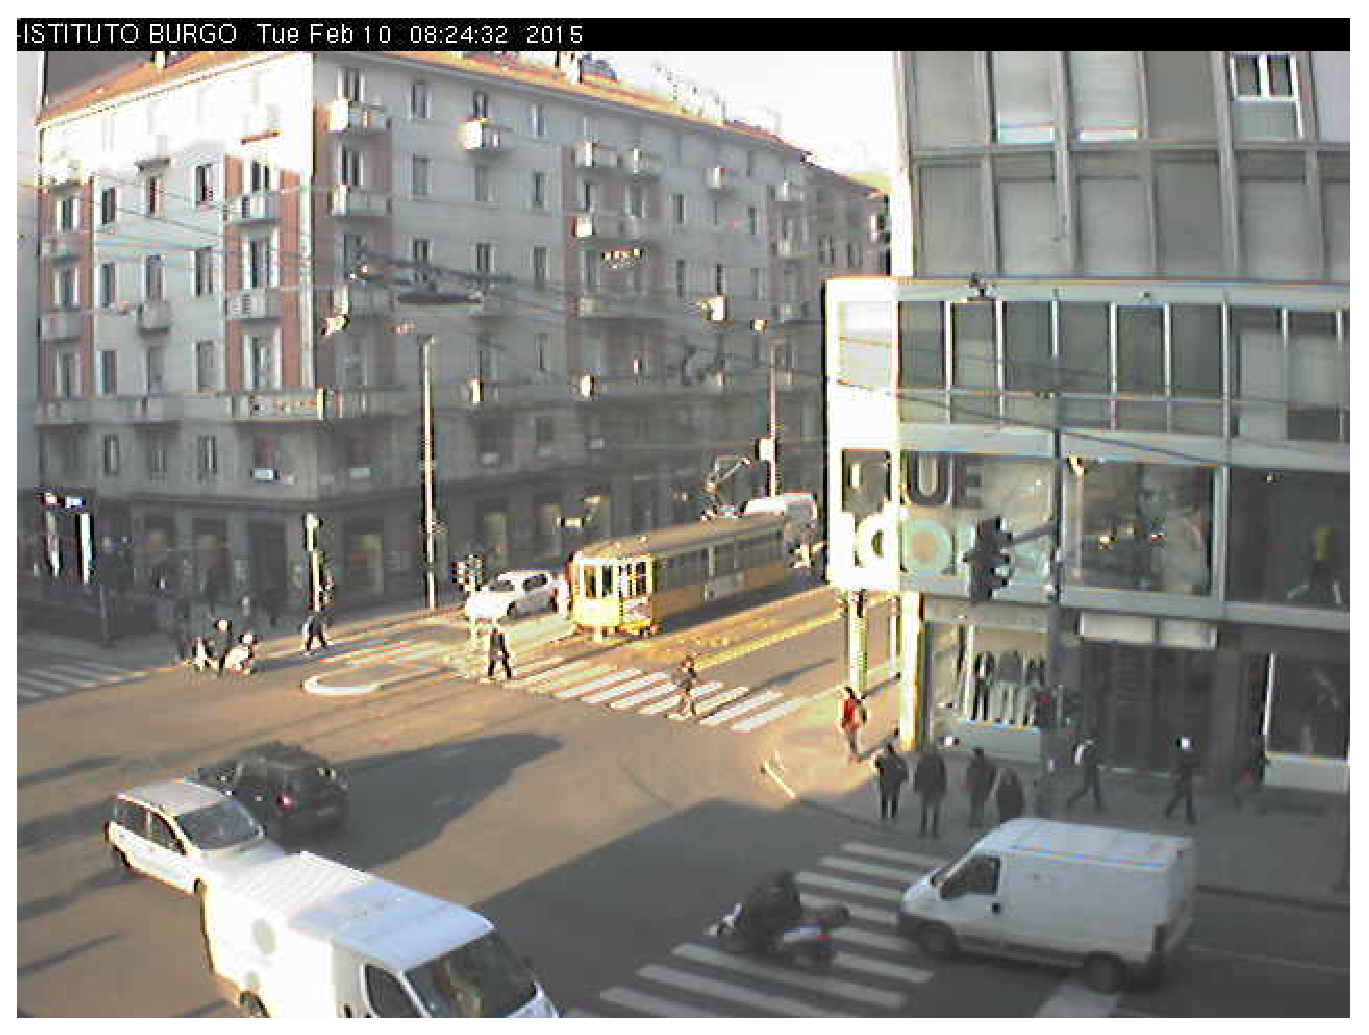
\includegraphics[width = 3cm]{./pictures/FPSbasso/image2692}
	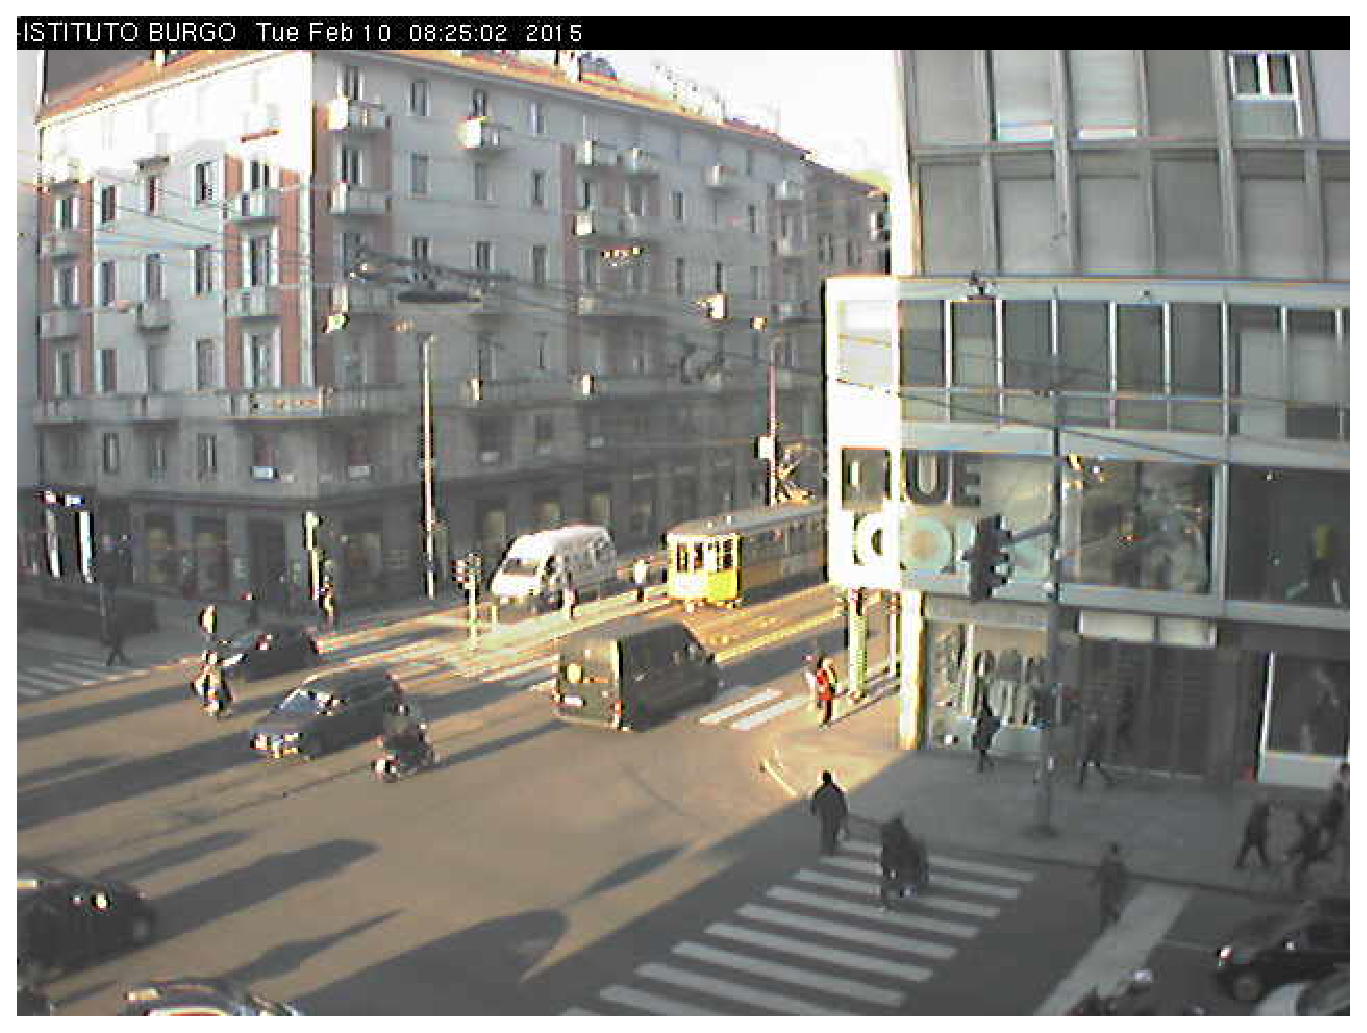
\includegraphics[width = 3cm]{./pictures/FPSbasso/image2693}
	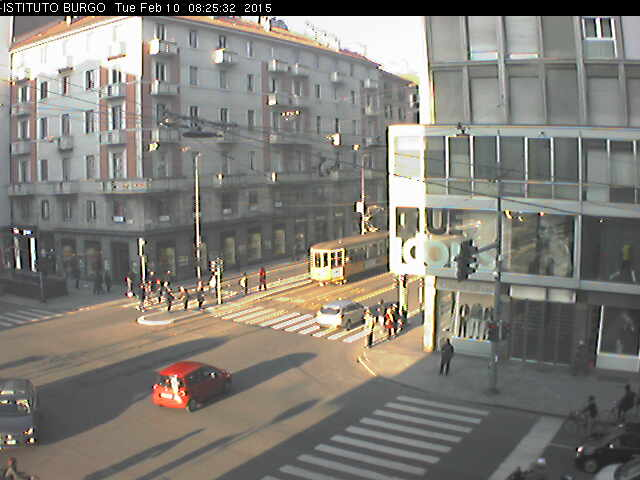
\includegraphics[width = 3cm]{./pictures/FPSbasso/image2694}
	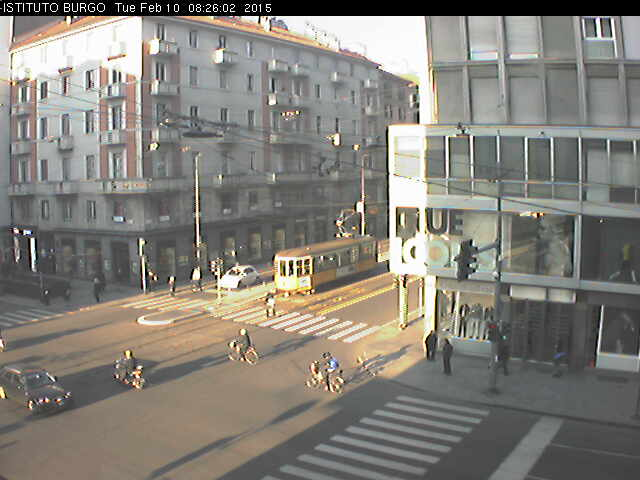
\includegraphics[width = 3cm]{./pictures/FPSbasso/image2695}
	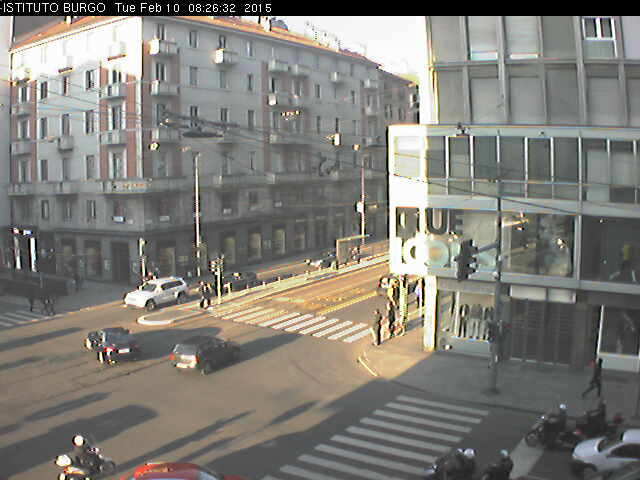
\includegraphics[width = 3cm]{./pictures/FPSbasso/image2696}
	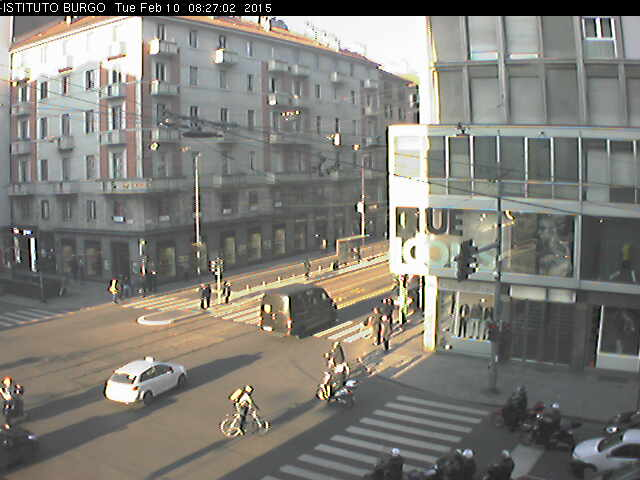
\includegraphics[width = 3cm]{./pictures/FPSbasso/image2697}
	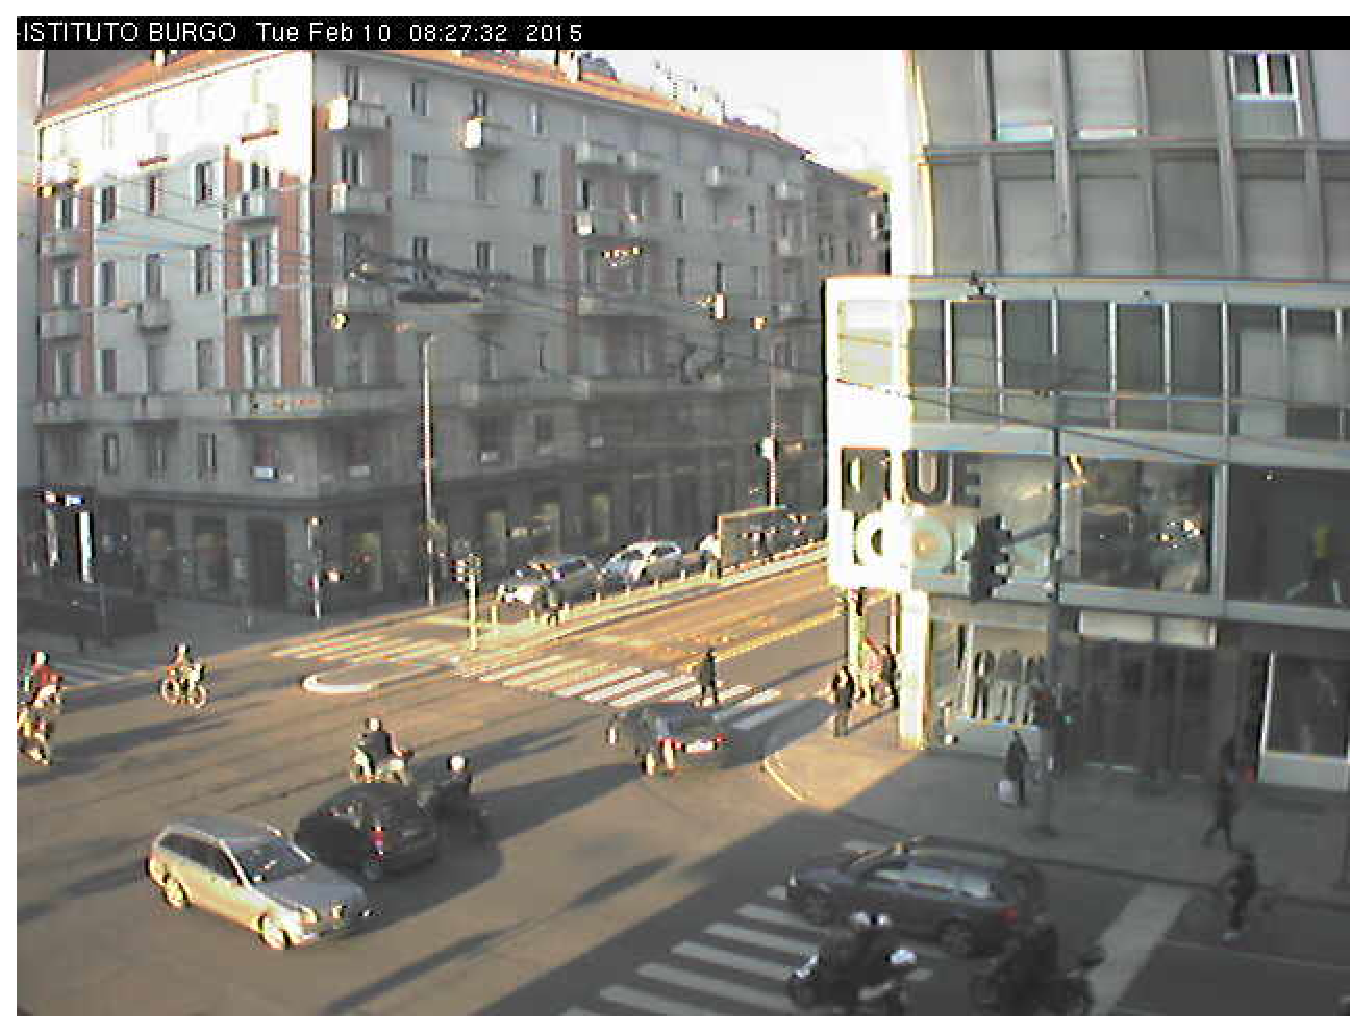
\includegraphics[width = 3cm]{./pictures/FPSbasso/image2698}
	\caption{Sequenza di frame acquisiti ogni 30 secondi}
	\label{fig:acquisizioneBassa}
\end{figure}
La figura \ref{fig:acquisizioneContinua} mostra come, in un'acquisizione fatta a 30 fps, le differenze tra frame consecutivi siano quasi inesistenti. 
Un evento di tampering pu\`o, quindi, essere identificato in maniera molto semplice, in quanto una differenza molto elevata tra il frame analizzato e il background pu\`o essere dovuto solamente a un'azione sulla camera.
La figura \ref{fig:acquisizioneBassa} mostra, invece, un esempio di frame acquisiti ogni 30 secondi.
Notiamo come le differenze tra immagini consecutive, in questo caso, siano pi\`u marcate rispetto al caso dell'acquisizione continua. 
Questo fa s\`i che l'utilizzo di un modello di background risulti inefficiente.
Evidenziamo, inoltre, come le tecniche viste finora richiedano capacit\`a computazionale da parte del sistema di monitoraggio.\\
Un approccio alternativo consiste nel monitorare nel tempo il comportamento di alcuni indicatori estratti dalle singole immagini acquisite.
Si presuppone che, quando il sistema di monitoraggio opera in condizioni di funzionamento \textit{ottimali}, gli indicatori monitorati presentino una certa \textit{stazionariet\`a}, ovvero siano considerati dei campioni \textit{indipendenti} tra loro e distribuiti secondo una stessa funzione di ripartizione.
L'evento di tampering viene considerato come un \textit{cambiamento nella stazionariet\`a} di questi indicatori.\\
Il monitoraggio pu\`o avvenire utilizzando tecniche statistiche, come ad esempio \textit{change-point method} (CPM) \cite{ross2011nonparametric} o \textit{change-detection test} \cite{pimentel2014review}.
Troviamo alcuni esempi nell'identificazione di sfocature: in \cite{tsesmelis2013tamper} la soluzione consiste nel monitorare nel tempo il \textit{numero di SURF} \cite{bay2006surf}, in quanto tali descrittori decrementano in maniera considerevole il loro numero in presenza di sfocature.
Notiamo, per\`o, che l'utilizzo di una tecnica del genere richiede un elevato numero di calcoli per ricavare le SURF.
Il metodo, quindi, si presta poco a essere utilizzato su sistemi di monitoraggio a basso consumo.
Un altro esempio \`e dato da \cite{alippi2010detecting}, dove le sfocature vengono identificate monitorando l'\textit{energia media del gradiente} delle immagini acquisite:
\begin{equation}
\label{eq:energyGradient}
m_i = \mathcal{M}[z_i] = \int_{\mathcal{X}}\| \bigtriangledown z_i(x) \| _1 dx,
\end{equation}  
dove $\| \cdot \|_1$ si riferisce alla \textit{norma} $\mathcal{L}^1$. 
Per identificare il cambio di stazionariet\`a di questo indicatore vengono utilizzate tecniche di CDT basate su \textit{somme cumulate} (CUSUM) \cite{alippi2008just}, utilizzando un sottoinsieme delle prime osservazioni come sequenza di \textit{training}, utilizzata per configurare il test.